\documentclass[11pt]{book}
    \usepackage{amsmath,amsfonts,amssymb,amsthm}
    \usepackage{tikz}
\usetikzlibrary{arrows.meta,bending,matrix,positioning}

    \begin{document}
\begin{equation}
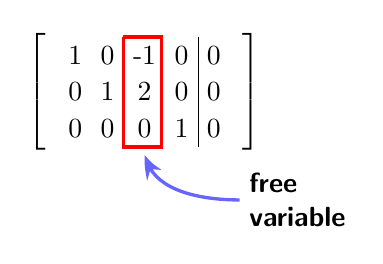
\begin{tikzpicture}[
    node distance=1mm and 0mm,
    baseline]
\matrix (M1) [matrix of nodes,{left delimiter=[},{right delimiter=]}]
{
  1 & 0 & -1 & 0 & 0 \\
  0 & 1 & 2  & 0 & 0 \\
  0 & 0 & 0  & 1 & 0 \\
};
\draw   (M1-1-4.north east) -- (M1-3-4.south east);
\draw[red,very thick]
        (M1-1-3.north west) -| (M1-3-3.south east) -| (M1-1-3.north west);
\node (fv) [below right=of M1.south east,align=left,
            font=\sffamily\bfseries] {free\\variable};
\draw[blue!60,very thick,shorten >=1mm,-{Stealth[bend]}]
        (fv.west) to [out=180,in=270] (M1-3-3.south);
\end{tikzpicture}
\end{equation}
    \end{document}
